\section{Lösungskonzept}
\textcolor{red}{Zum Schluss der Arbeit kann in dem letzten Teil eine thesenartige Zusammenfassung der Untersuchungsergebnisse gegeben werden. Andere Möglichkeiten sind hier auch der Ausblick auf weitere – noch ungelöste – Fragestellungen im Zusammenhang mit dem Thema.}

\subsection{Zielarchitektur}
Hier die Standard-Architektur-Modell von SAP


  \begin{figure}[H]
    \centering
    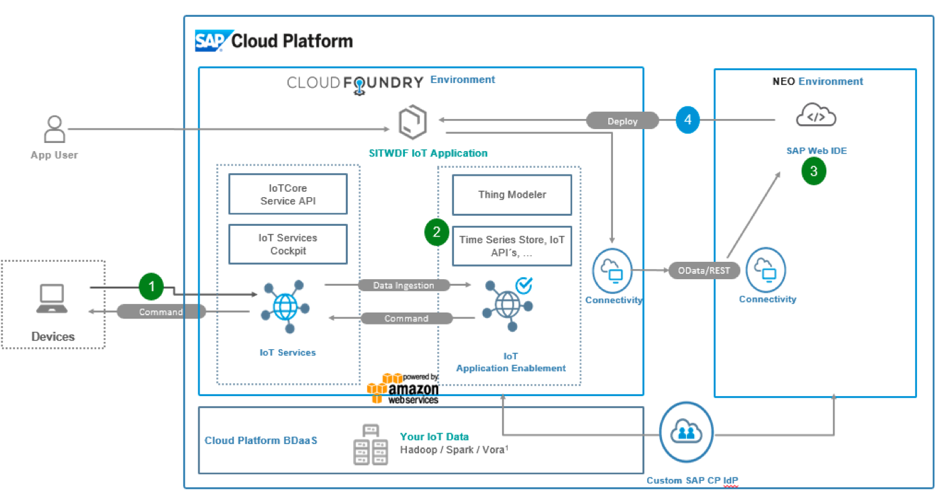
\includegraphics[width=1.0\linewidth]{pictures/sap_architecture}
    \caption[Referenzarchitektur von SAP]{Architektur von SAP \citep{Ganz2019}}
    \label{fig:filename_without_extension}
  \end{figure}


\subsubsection{SAP Cloud Platform}

SAP Cloud Platform und AWS Microservices und APIs
Programmiersprachen und Laufzeitumgebungen
CF, NEO, ABAP
Destinations

\subsubsection{SAP Leonardo}
Innovationsplattform
GUI, API, SDKs
\subsubsection{AWS Cloud}
SNS-Server

\subsection{Kommunikation}

\subsubsection{MQTT}

\subsubsection{REST}

\subsubsection{Edge-Processing}

\subsubsection{Destinations}
Destinations: Warum braucht man Destinations und welche man benötigt (SNS),  wenn man kommunizieren will mit
Externe Services wie AWS SNS
Interne Kommunikation der SCP CF und NEO
Communication zwischen Cloud Services AWS SNS und SAP Leonardo

\subsubsection{Message Processing}
Leonardo IoT, SQL Kafka: Ich hab Leonardo IoT benutzt (in prototype erwähnen)

\subsection{Sicherheit}
OAuth, SSL/TLS, SAML 2.0: erklären, was SAP und AWS auch eventuell haben

